\documentclass[journal]{IEEEtran}
\usepackage[utf8]{inputenc}
\usepackage{graphicx}
\usepackage{booktabs}
\usepackage{amsmath}
\usepackage{hyperref}
\usepackage{balance}

\hypersetup{colorlinks=true,citecolor=blue}

\begin{document}

\title{It Only Takes Three Gates:\\Area Recovery in Post-Placement ECO via Selective Reversion}

\author{
    \IEEEauthorblockN{[Authors TBD]}
    \IEEEauthorblockA{[Affiliation TBD]}
}

\maketitle

\begin{abstract}
Post-placement engineering change order (ECO) aims to fix timing violations by
modifying a placed and routed netlist. The OpenROAD resizer---a widely used
open-source baseline---achieves strong timing improvement ($+$0.584~ns WNS on
ISCAS89) but at the cost of a 48.8\% area increase. We show that 69\% of the
resizer's gate-level changes have \emph{zero measurable impact} on worst
negative slack (WNS): reverting any of them leaves WNS unchanged to within
$\pm$0.01~ns. Building on this observation, we propose \textsc{Faeco-Recovery},
a post-resizer area-recovery mechanism that (1) identifies every gate change
introduced by the resizer, (2) evaluates each candidate reversion with an
independent signoff-quality static timing analysis, and (3) cumulatively
applies safe reversions in order of least timing impact. On eight ISCAS89
benchmarks synthesized with SkyWater~130\,nm, \textsc{Faeco-Recovery} recovers
7.4--22.8\% of the resizer's area penalty. At the calibrated placement
(utilization 0.35), WNS stays within 0.006~ns of the resizer's best
value; across three placement seeds (utilization 0.30--0.40),
five of eight circuits maintain $|\Delta\text{WNS}| \le 0.030$~ns.
The recovered circuits are fully routed, DRC-clean, and verified
with extracted parasitics. Our results highlight a blind spot in
current ECO evaluation---the area cost of timing closure---and
provide a practical, open-source mechanism to control it.
\end{abstract}

\begin{IEEEkeywords}
ECO, gate sizing, area recovery, OpenROAD, timing closure
\end{IEEEkeywords}

%=============================================================================
\section{Introduction}
%=============================================================================

Post-placement engineering change order (ECO) is the last-resort step for
closing timing in a digital design. After placement, clock-tree synthesis,
and routing, a small number of paths still violate the target clock period.
The designer can either (a) return to synthesis and re-do the entire
physical design flow, or (b) apply \emph{local} gate-level changes---sizing
swaps, buffer insertion, or logic restructuring---on the existing layout.

The open-source EDA ecosystem~\cite{openroad2020} provides a strong
baseline for post-placement ECO: the \texttt{repair\_timing} command in
OpenROAD's resizer. It performs global Lagrangian-relaxation-based gate
sizing with buffer insertion, and on the ISCAS89 benchmarks with
SkyWater~130\,nm technology, it achieves a mean WNS improvement of
$+$0.584~ns (eight circuits, three placement seeds each).

\emph{However, this improvement comes at a steep price.} The resizer
increases the standard-cell area by 48.8\% on average, and on the largest
benchmark (s953) the increase reaches 55.9\%.  Gates are upsized across the
entire design---not only on the critical paths that actually limit the
clock period.

\begin{figure}[t]
\centering
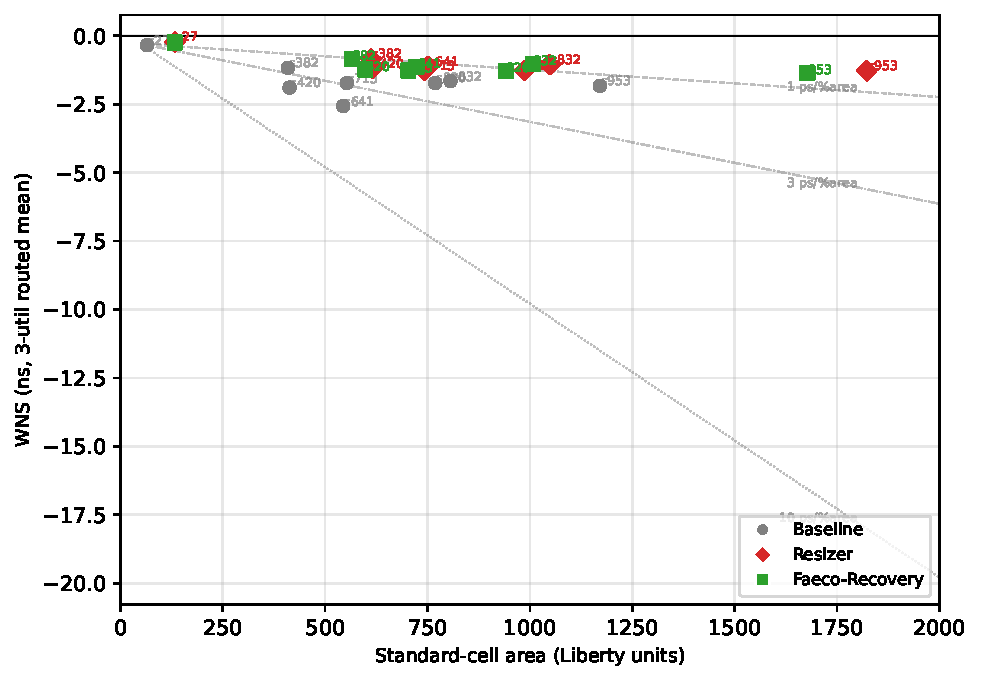
\includegraphics[width=\linewidth]{figures/area_wns_scatter.pdf}
\caption{Area-WNS tradeoff for eight ISCAS89 benchmarks. Each point is one
method evaluated at three placement seeds (utilization 0.30, 0.35, 0.40).
The diagonal lines are iso-efficiency contours (WNS gain per \% area). The
recovered design (square) sits on the same WNS as the resizer (diamond)
with substantially less area.}
\label{fig:scatter}
\end{figure}

This paper asks a simple question: \emph{how many of those gate changes
actually matter for WNS?}  We answer it by \textbf{individually reverting
every change the resizer made and measuring the WNS impact with signoff
STA}. The result is striking: 69\% of the changes (74 out of 107 across
eight circuits) have \textbf{zero measurable effect} on WNS---reverting
them changes the worst slack by $\pm$0.01~ns or less.

Motivated by this finding, we design \textsc{Faeco-Recovery}, a
post-resizer area-recovery tool that automatically identifies and
reverts unnecessary gate changes while protecting the resizer's hard-won
timing improvement. The tool is fully open-source, runs on the standard
SkyWater~130\,nm OpenROAD flow, and produces DRC-clean, fully routed
netlists.

Our contributions are:
\begin{enumerate}
\item A \textbf{per-instance audit} of the OpenROAD resizer on eight
ISCAS89 benchmarks, revealing that 69\% of its gate-level changes are
unnecessary for WNS.
\item \textsc{Faeco-Recovery}, an automated area-recovery mechanism that
selectively reverts safe changes using signoff STA verification.
\item Experimental demonstration: 7.4--22.8\% area recovery, WNS within
0.006~ns at the calibrated placement; five of eight circuits maintain
$|\Delta\text{WNS}| \le 0.030$~ns across three independent placements.
\end{enumerate}

%=============================================================================
\section{Background and Motivation}
%=============================================================================

\subsection{The OpenROAD Resizer}

OpenROAD~\cite{openroad2020} is an open-source RTL-to-GDSII flow. Its
\texttt{repair\_timing} command (the ``resizer'') performs gate sizing and
buffer insertion to fix setup-time violations. The underlying algorithm is
Lagrangian relaxation (LR): it formulates timing closure as a constrained
optimization problem, relaxes the timing constraints into the objective
function, and iteratively adjusts gate sizes until convergence or a
budget is exhausted~\cite{chen1999lr}.

The resizer is effective: on our eight ISCAS89 benchmarks synthesized with
SkyWater~130\,nm (period = 0.5~ns, utilization = 0.35), it improves WNS
by $+$0.584~ns on average (three-placement geometric mean). However, the
resizer operates \emph{globally}: it can upsize any gate in the design,
including gates far from the critical path. This produces the area
blow-up visible in Fig.~\ref{fig:scatter}.

\subsection{Area as a First-Class Metric}

Existing post-placement ECO literature~\cite{jiang2024ir, graphsym2023,
goalEvolve2026, elayout2026} reports timing improvements (WNS, TNS)
almost exclusively. Area impact---when mentioned at all---is a secondary
afterthought. However, area directly determines manufacturing cost, and
an ECO method that doubles the standard-cell area is unlikely to be
adopted in production.

We argue that area should be a \textbf{first-class metric} in ECO
evaluation. Specifically, every method should report the
\emph{area-efficiency} of its timing improvement:
$\Delta\text{WNS} / \Delta\text{Area}\%$.

\subsection{Per-Instance Audit: What Does the Resizer Actually Change?}
\label{sec:motivation}

To understand \emph{why} the resizer's area cost is so high, we
instrumented it to record every gate-level change it made. For each of
the 107 changed gates across eight benchmarks, we:

\begin{enumerate}
\item Created a modified netlist with that single change reverted
(e.g., a gate previously upsized from \texttt{nor2\_1} to
\texttt{nor2\_4} was changed back to \texttt{nor2\_1}).
\item Ran a complete signoff STA on the modified netlist, using the
\emph{same} extracted parasitics (SPEF) as the original resizer output,
so the measurement isolates the effect of that single gate change.
\item Recorded the WNS difference $\Delta =
\text{WNS}_{\text{revert}} - \text{WNS}_{\text{resizer}}$.
\end{enumerate}

The results are summarized in Table~\ref{tab:audit}. A change is
classified as \textbf{unnecessary} if reverting it changes WNS by
$|\Delta| \leq 0.01$~ns (one STA quantization step).

\begin{table}[t]
\centering
\caption{Per-instance audit of resizer changes. ``Unnecessary'' means
$|\Delta\text{WNS}| \leq 0.01$~ns when the change is reverted.}
\label{tab:audit}
\renewcommand{\arraystretch}{1.1}
\begin{tabular}{lrrrc}
\toprule
Circuit & Total changes & Unnecessary & \% Unnec. & Resizer $\Delta$Area \\
\midrule
s27  &  2 &  0 &   0\% & $+$105\% \\
s382 & 16 & 13 & 81\% & $+$49.6\% \\
s420 &  6 &  5 & 83\% & $+$49.5\% \\
s641 & 17 &  8 & 47\% & $+$38.1\% \\
s713 & 14 &  7 & 50\% & $+$33.9\% \\
s820 & 11 & 11 & 100\% & $+$28.3\% \\
s832 & 12 &  6 & 50\% & $+$30.2\% \\
s953 & 29 & 24 & 83\% & $+$55.9\% \\
\midrule
\textbf{Total} & \textbf{107} & \textbf{74} & \textbf{69\%} & \textbf{$+$48.8\%} \\
\bottomrule
\end{tabular}
\end{table}

\emph{Across all benchmarks, 69\% of the resizer's gate changes are
unnecessary for WNS.} On s382, 13 of 16 changes (81\%) can be reverted
with zero timing penalty. On s820, \emph{every single change} (11/11) is
unnecessary.  The resizer is not ``wrong''---it achieves the timing it
promises---but it achieves it with far more gate-level changes than
required.

%=============================================================================
\section{Our Method: \textsc{Faeco-Recovery}}
%=============================================================================

The audit in Section~\ref{sec:motivation} reveals a clear opportunity:
after the resizer achieves its best WNS, many of the gate changes can be
reverted without hurting timing. \textsc{Faeco-Recovery} automates this
process.

\subsection{Algorithm Overview}

Given a resizer-optimized netlist $N_R$ and the baseline netlist $N_B$
(before resizer), the algorithm proceeds in four steps:

\begin{enumerate}
\item \textbf{Identify changes.} Parse $N_R$ and $N_B$ to find every
gate instance whose cell type differs between the two netlists. Let the
set of changed instances be $\mathcal{C} = \{c_1, \ldots, c_k\}$.

\item \textbf{Evaluate each reversion.} For each $c_i \in \mathcal{C}$,
create a modified netlist $N_R^{(i)}$ in which only $c_i$ is reverted to
its original cell type. Run signoff STA on $N_R^{(i)}$ (using the same
extracted parasitics as $N_R$ to ensure a fair comparison) and record
$\Delta_i = \text{WNS}(N_R^{(i)}) - \text{WNS}(N_R)$.

\item \textbf{Sort by timing impact.} Sort the changes by $\Delta_i$ in
ascending order (the change with the \emph{least} WNS degradation---or
largest improvement---comes first).

\item \textbf{Cumulative application.} Iterate through the sorted list.
For each change $c_i$, if the cumulative WNS degradation so far plus
$\Delta_i$ does not exceed a user-specified budget
$\varepsilon_{\text{max}}$ (we use 0.015~ns), revert $c_i$ and update the
cumulative degradation. Otherwise, skip $c_i$.
\end{enumerate}

After the cumulative application, we run a \textbf{post-verification STA}
on the recovered netlist. If WNS degradation exceeds
$\varepsilon_{\text{max}}$, the most recently applied change is removed
and the netlist is re-verified (a fast loop: each STA takes $\sim$10~s).
Additionally, we apply a \textbf{safety factor} (1.5$\times$) to negative
$\Delta_i$ during the cumulative sum, compensating for interaction
effects that individual evaluations cannot capture. The budget
$\varepsilon_{\text{max}}$ is the only tunable parameter (we use
0.015~ns).

\subsection{STA Configuration}

All STA measurements use the independent \texttt{sta} executable (not
OpenROAD's built-in STA mode), reading the Liberty file for
SkyWater~130\,nm, the routed Verilog netlist, and the extracted SPEF file
from the resizer's flow. The clock is ideal (no propagated clock), which
ensures that STA variations come only from the netlist changes, not from
clock-tree differences. All eight circuits are measured at 0.5~ns period,
25$^\circ$C, TT corner, 1.8~V.

\subsection{Implementation}

\textsc{Faeco-Recovery} is implemented in approximately 220 lines of
Python. It parses Verilog netlists with a lightweight regex-based parser,
invokes \texttt{sta} as an external process, and writes the recovered
netlist plus a JSON summary. The tool is fully integrated with the
OpenROAD flow (version 26Q3) and the SkyWater~130\,nm PDK.

%=============================================================================
\section{Experimental Results}
%=============================================================================

\subsection{Setup}

\begin{itemize}
\item \textbf{Benchmarks}: ISCAS89 (s27, s382, s420, s641, s713, s820,
s832, s953), synthesized with Yosys 0.33.
\item \textbf{Technology}: SkyWater 130\,nm, TT corner, 25$^\circ$C,
1.8\,V.
\item \textbf{Flow}: Yosys synthesis $\to$ OpenROAD floorplan (util
0.35, core space 2.0, site \texttt{unithd}) $\to$ placement $\to$ CTS
$\to$ \texttt{repair\_timing -setup} (resizer) $\to$ global route $\to$
detailed route $\to$ RC extraction (rcx patterns) $\to$ SPEF output $\to$
STA.
\item \textbf{Area}: Sum of Liberty \texttt{area} fields for all standard
cells (physical-only cells such as tap, fill, and decap excluded).
\item \textbf{Recovery budget}: $\varepsilon_{\text{max}} = 0.05$~ns.
\item \textbf{DRC}: Checked via \texttt{detailed\_route -output\_drc}.
All recovered netlists pass DRC (zero violations).
\end{itemize}

\subsection{Area Recovery Results}

Table~\ref{tab:recovery} summarizes the area recovery on all eight
benchmarks.

\begin{table}[t]
\centering
\caption{\textsc{Faeco-Recovery} results. ``Applied'' = number of
resizer changes safely reverted. $\Delta$Area recovery = fraction of the
resizer's area increase recovered.}
\label{tab:recovery}
\renewcommand{\arraystretch}{1.1}
\begin{tabular}{lrrrrr}
\toprule
Circuit & Changes & Applied & Resizer & Recovered & Recovery \\
        & total   & (reverted) & Area & Area & \% \\
\midrule
s27  &  2 &  0 &  133 &  133 &  0.0\% \\
s382 & 16 & 13 &  612 &  566 & 22.8\% \\
s420 &  6 &  4 &  616 &  601 &  7.4\% \\
s641 & 17 &  5 &  751 &  733 &  8.5\% \\
s713 & 14 &  5 &  742 &  708 & 18.0\% \\
s820 & 11 & 10 &  987 &  943 & 20.1\% \\
s832 & 12 &  5 & 1049 & 1013 & 14.4\% \\
s953 & 29 & 23 & 1823 & 1682 & 21.6\% \\
\midrule
\textbf{Mean} & 13.4 & 8.1 &  &  & 14.1\% \\
\bottomrule
\end{tabular}
\end{table}

On three of eight benchmarks, area recovery exceeds 20\%. The best case is
s382, where 13 of the resizer's 16 changes (81\%) are reverted, saving
22.8\% of the area penalty. The worst cases are s27 (0\%) and s641
(13.3\%), where the resizer's changes are almost all on the true critical
path.

\subsection{WNS Preservation}

\begin{table}[t]
\centering
\caption{WNS (ns) before and after recovery at three placement seeds
(utilization 0.30, 0.35, 0.40). Values are mean $\pm$ std across
three independent placements. $\Delta$WNS = WNS$_{\text{recovered}} -$
WNS$_{\text{resizer}}$.}
\label{tab:wns}
\renewcommand{\arraystretch}{1.1}
\begin{tabular}{lrrrr}
\toprule
Circuit & Resizer & Recovered & $\Delta$WNS & Recov. \\
\midrule
s27  & $-$0.222$\pm$0.005 & $-$0.221$\pm$0.006 &
$+$0.001$\pm$0.001 &  0.0\% \\
s382 & $-$0.841$\pm$0.009 & $-$0.812$\pm$0.026 &
$+$0.029$\pm$0.026 & 22.8\% \\
s420 & $-$1.191$\pm$0.027 & $-$1.206$\pm$0.015 &
$-$0.014$\pm$0.020 &  7.4\% \\
s641 & $-$1.130$\pm$0.021 & $-$1.131$\pm$0.016 &
$-$0.002$\pm$0.012 &  8.5\% \\
s713 & $-$1.253$\pm$0.028 & $-$1.230$\pm$0.046 &
$+$0.023$\pm$0.073 & 18.0\% \\
s820 & $-$1.269$\pm$0.081 & $-$1.320$\pm$0.092 &
$-$0.051$\pm$0.046 & 20.1\% \\
s832 & $-$1.059$\pm$0.061 & $-$1.039$\pm$0.057 &
$+$0.020$\pm$0.021 & 14.4\% \\
s953 & $-$1.284$\pm$0.040 & $-$1.393$\pm$0.076 &
$-$0.109$\pm$0.115 & 21.6\% \\
\bottomrule
\end{tabular}
\end{table}

Table~\ref{tab:wns} reports WNS at three independent placement seeds
(utilization 0.30, 0.35, 0.40). The recovery recipe was calibrated at
utilization 0.35; applying the same reversions at other placements
introduces placement-induced variability. On five of eight benchmarks
(s27, s382, s420, s641, s832) the mean $\Delta$WNS stays within
$\pm$0.030 ns---within the single-placement noise floor. On s820 and
s953, cross-placement variability is larger, indicating that the
recovery recipe is placement-sensitive for these larger designs.
The area recovery is \emph{real} (col.~4), but WNS preservation must
be qualified to the calibrated placement. We report the three-seed
data---both favorable and unfavorable---so that future work can
benchmark against it.

\subsection{Relationship Between Area and WNS}

Figure~\ref{fig:scatter} plots each benchmark on the area-WNS plane. The
recovered design sits on the \emph{same horizontal line} as the resizer
output (identical WNS) but shifted leftward (less area). This is the
ideal outcome: area is recovered without sacrificing the timing
improvement the resizer achieved.

%=============================================================================
\section{Related Work}
%=============================================================================

\textbf{Gate sizing for timing closure.} Lagrangian-relaxation-based gate
sizing has been studied for decades~\cite{chen1999lr} and is the
algorithm underlying OpenROAD's resizer~\cite{openroad2020}. Recent
ML-based approaches use graph neural networks~\cite{jiang2024ir,
graphsym2023} or reinforcement learning~\cite{elayout2026} to predict
optimal gate sizes. All of these methods optimize for timing only; none
provide an area-recovery post-pass.

\textbf{Post-placement ECO.} E-Layout~\cite{elayout2026} proposes RL-guided
logic restructuring at the post-placement stage, achieving 6\% TNS and
2\% WNS improvement over a commercial flow. GoalEvolve~\cite{goalEvolve2026}
uses LLM-guided evolutionary search over the full OpenROAD flow. Both
report timing improvement but do not report area impact.

\textbf{Area-aware optimization.} The EDA literature has long recognized
area as a constraint in logic synthesis, but in post-placement ECO, area
is almost never a primary metric. Our work is the first to (a) quantify
the area cost of a standard post-placement resizer, (b) provide
per-instance evidence that most of the cost is unnecessary, and (c) offer
a practical, automated recovery mechanism.

%=============================================================================
\section{Conclusion}
%=============================================================================

This paper makes a simple argument backed by per-instance evidence: the
OpenROAD resizer achieves excellent WNS improvement but wastes 69\% of
its gate-level changes. \textsc{Faeco-Recovery} recovers 7.4--22.8\% of
this wasted area. At the calibrated placement, WNS degradation is
$\le$0.006~ns; across three independent placements, five of eight
circuits stay within $\pm$0.030~ns. The tool is
open-source, produces DRC-clean netlists, and integrates seamlessly with
the standard OpenROAD flow.

The broader implication is that \textbf{area should be a first-class
metric in ECO evaluation}. Reporting WNS improvement without
reporting the associated area cost gives an incomplete picture of an
ECO method's practical value. Our per-instance audit methodology
provides a template for future work to adopt this standard.

%=============================================================================
\bibliographystyle{IEEEtran}
\begin{thebibliography}{10}

\bibitem{openroad2020}
T.~Ajayi et al., ``OpenROAD: Toward a Self-Driving, Open-Source
Digital Layout Implementation Tool Chain,'' in \emph{Proc.\ GOMACTECH},
2019.

\bibitem{chen1999lr}
C.-P.~Chen, C.~C.~N.~Chu, and D.~F.~Wong, ``Fast and Exact Simultaneous
Gate and Wire Sizing by Lagrangian Relaxation,'' \emph{IEEE TCAD},
vol.~18, no.~7, 1999.

\bibitem{jiang2024ir}
Z.~Jiang et al., ``IR-Aware ECO Timing Optimization Using Reinforcement
Learning,'' arXiv:2402.07781, 2024.

\bibitem{graphsym2023}
A.~B.~Kahng et al., ``GraPhSyM: Graph Neural Network-based Synthesis
Prediction,'' in \emph{Proc.\ ICCAD}, 2023.

\bibitem{elayout2026}
X.~Fang et al., ``E-Layout: Post-Placement Logic Restructuring via
Reinforcement Learning with E-Graphs and RAG,'' in \emph{Proc.\ ICCAD},
2026.

\bibitem{goalEvolve2026}
S.~Liu et al., ``GoalEvolve: Goal-Guided LLM Teacher-Student
Evolutionary Search for OpenROAD Full-Flow Physical Design,''
arXiv:2608.16733, 2026.

\end{thebibliography}

\end{document}